\documentclass{article}
\usepackage[utf8]{inputenc}
\usepackage{graphicx}
\usepackage{wrapfig}
\usepackage[T1]{fontenc}
\usepackage{amssymb}
\usepackage{siunitx}
\usepackage{gensymb}

\title{Steady- State Performance of a 1-Phase Transformer}
\author{Aditya Agrawal\\2021AM10198\\GROUP 29}
\date{June 4, 2022}

\begin{document}
\maketitle
\tableofcontents
\newpage
\section{Single Phase Transformer}
\subsection{Aim}
Obtain equivalent circuit parameters by conducting open-circuit, short-circuit
and resistance measurement tests.
\subsection{Apparatus Required}
\begin{enumerate}
    \item 1-Phase Transformer of identical ratings
    \item 1-Phase Auto-transformer
    \item AC Ammeter
    \item AC Voltmeter
\end{enumerate}
\subsection{Theory}
\begin{wrapfigure}{R}{0.2\textwidth}
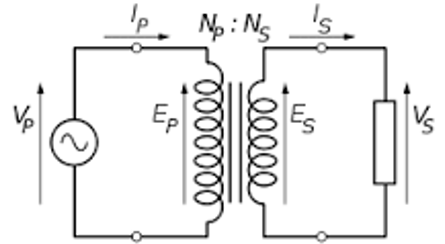
\includegraphics[width=0.3\textwidth]{img1.png}
\end{wrapfigure}
A single phase transformer consists of two magnetically coupled windings that are capable of transforming the voltage and current of an alternating supply to different values. Two windings, one referred to as the input or primary winding and the other as the output or secondary winding, are placed on a silicon steel-stamped core. The core provides a path with low reluctance for the magnetic flux that connects the two windings.\par
If we assume the pulsating flux $\Phi$ to have a sinusoidal waveform $\Phi_{m}$Cos$\omega$ t, where $\omega$ is the supply frequency in radians per second, the induced primary voltage is given by:\\
\begin{equation}
    E_{1} = -N_{1}\frac{d\Phi_{m}}{dt}
\end{equation}
where $N_{1}$ is the number of primary turns.\par
Thus the primary RMS induced voltage $E_{1}$ is proportional to the primary turns $N_{1}$ and 
lags behind the flux by 90$\degree$. Since the flux $\Phi_{m}$ also links with the secondary turns and is in phase with $E_{1}$.\\
\begin{equation}
    \frac{E_{1}}{E_{2}}=\frac{N_{1}}{N_{2}}
\end{equation}
Now, $E_{1}$ opposes the applied voltage say $V_{I}$ and is nearly equal to $V_{I}$ if the primary 
resistance and leakage reactance is very small.\par
Now with the primary resistance and leakage inductance neglected, we have:
\begin{equation}
    E_{1}=V_{1}
\end{equation}
\begin{equation}
    E_{2}=V_{2}
\end{equation}
Since $E_{2}$/$E_{1}$ = $N_{2}$/$N_{1}$, we can say that $V_{2}$/$V_{1}$ = $N_{2}$/$N_{1}$. Thus approximately the output voltage bears the same ratio to the input voltage, which secondary turns bear to the primary 
turns.\par
Until now, the secondary has been deemed open circuit. Current $I_{2}$ will flow through the load and secondary winding if it is loaded. This current reduces the magnetic flux $\Phi_{m}$ in accordance with Lenz's law. This reduces the $E_{1}$ induced emf. Now, the current from the primary source rushes to cancel out the effect of the secondary current and establish flux $\Phi_{m}$ equilibrium. The mutual flux has therefore transferred power from the primary to the secondary winding. Now, ignoring losses, it is possible to state that output power equals input power.Thus:
\begin{equation}
    I_{2}E_{2}=I_{1}E_{1}
\end{equation}
\begin{equation}
    \frac{I_{2}}{I_{1}}=\frac{E_{1}}{E_{2}}=\frac{N_{1}}{N_{2}}
\end{equation}

Therefore the current ratio is equal to the inverse of the voltage turns ratio. This situation in 
the phasor diagram where $I_{2}$ is shown to balance the effect of $I_{2}$ and the total input current on load become $I_{1}$. The phasor diagram can now be modified to include the effect of resistance 
and leakage reactances of the windings.\par
\begin{figure}[h!]
    \centering
    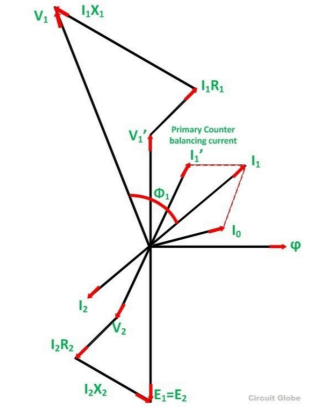
\includegraphics[width=0.5\textwidth]{img2.png}
    \caption{Full-load phasor diagram}
\end{figure}
It is seen that the open circuit test on transformer is used to determine core losses in transformer and parameters of shunt branch of the equivalent circuit
of transformer.\par
It is seen that the short circuit test on transformer is used to determine
copper loss in transformer at full load and parameters of approximate equivalent
circuit of transformer.
\subsection{Breadboard Setup}
\begin{figure}[h!]
    \centering
    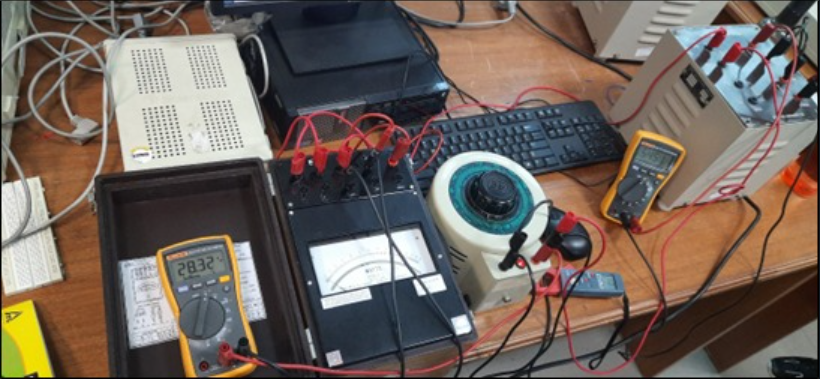
\includegraphics[width=0.7\textwidth]{img3.png}
    \caption{Open Circuit Test}
\end{figure}
\begin{figure}[h!]
    \centering
    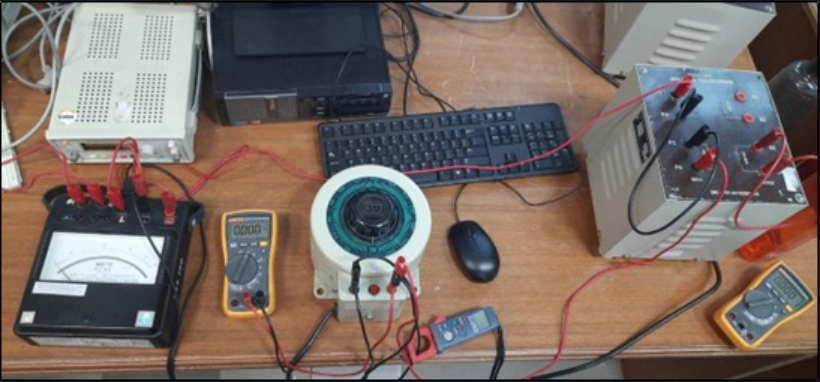
\includegraphics[width=0.7\textwidth]{img4.png}
    \caption{Short Circuit Test}
\end{figure}
\subsection{Observations}
\begin{center}
\textbf{Open Circuit Test}\\\vspace{2mm}
\begin{tabular}{|c|c|c|c|}
\hline
    $V_{Input}$(V) & Current(A) & Power(W) & $V_{Output}$(V) \\
    \hline
    28.29 & 0.11 & 1 & 54.54\\
    47.45 & 0.15 & 2.2 & 92.1\\
    68 & 0.19 & 4.2 & 133\\
    86.8 & 0.24 & 6.8 & 170.9\\
    107.4 & 0.33 & 9.7 & 210.5\\
    120 & 0.4 & 11.7 & 235.5\\
\hline
\end{tabular}
\newpage
\textbf{Short Circuit Test}\\\vspace{2mm}
\begin{tabular}{|c|c|c|}
\hline
    $V_{Input}$(V) & Current(A) & Power(W)\\
    \hline
    10.21 & 2.96 & 15 \\
    13.18 & 3.77 & 30\\
    16.8 & 4.79 & 65\\
\hline
\end{tabular}
\end{center}
\subsection{Calculations}
\subsubsection{Open Circuit Test}
\begin{center}
\begin{tabular}{|c|c|c|c|c|c|c|c|c|c|}
\hline
    $V_{0}$(V) & $I_{0}$(A) & $W_{0}$(W) & $V_{Out}$(V) & cos$\Phi_{0}$ & sin$\Phi_{0}$ & $I_{W}$ & $I_{\mu}$ & $R_{0}$ & $X_{0}$ \\
    \hline
    28.29 & 0.11 & 1.0 & 54.54 & 0.321 & 0.897 & 0.035 & 0.097 & 808.28 & 291.65\\
    47.45 & 0.15 & 2.2 & 92.1 & 0.309 & 0.904 & 0.046 & 0.136 & 1031.52 & 348.90\\
    68.00 & 0.19 & 4.2 & 133.0 & 0.325 & 0.890 & 0.062 & 0.169 & 1096.77 & 402.37\\
    86.8 & 0.24 & 6.8 & 170.9 & 0.326 & 0.894 & 0.078 & 0.215 & 1112.82 & 403.72\\
    107.4 & 0.33 & 9.7 & 210.5 & 0.273 & 0.925 & 0.090 & 0.305 & 1193.33 & 352.13\\
    120.00 & 0.4 & 11.7 & 235.5 & 0.243 & 0.941 & 0.097 & 0.376 & 1237.11 & 319.14\\
\hline
\end{tabular}
\end{center}
\vspace{2mm}
Hence,
\begin{itemize}
    \item $I_{W}$=$I_{0}$cos$\Phi_{0}$=0.068A
    \item $I_{\mu}$=$I_{0}$sin$\Phi_{0}$=0.216A
    \item $R_{0}$=$\frac{V_{0}}{I_{W}}$=1079.97$\Omega$
    \item $X_{0}$=$\frac{V_{0}}{I_{\mu}}$=352.99$\Omega$
\end{itemize}

\subsubsection{Short Circuit Test}
\vspace{1mm}
\begin{center}
    \begin{tabular}{|c|c|c|c|c|c|}
\hline
    $V_{SC}$(V) & $I_{SC}$(A) & $W_{SC}$(W) & $Z_{2}$($\Omega$) & $R_{2}$($\Omega$) & $X_{2}$($\Omega$)\\
    \hline
    10.21 & 2.96 & 15 & 3.449 & 1.712 & 2.994\\
    13.18 & 3.77 & 30 & 3.496 & 2.111 & 2.787\\
    16.8 & 4.79 & 65 & 3.507 & 2.851 & 2.042\\
\hline
\end{tabular}
\end{center}
\vspace{3mm}
Hence,
\begin{itemize}
    \item $Z_{2}$=$\frac{V_{SC}}{I_{SC}}$=3.484$\Omega$
    \item $R_{2}$=$\frac{W_{SC}}{I_{SC}^2}$=2.225$\Omega$
    \item $X_{2}$=$\sqrt{Z_{2}^2 - R_{2}^2}$=2.681$\Omega$
    \item $R_{1}$=$R_{2}$ $\times$ ($\frac{N_{1}}{N_{2}}$)=2.225$\Omega$
    \item $X_{1}$=$X_{2}$ $\times$ $(\frac{N_{1}}{N_{2}})^2$=2.681$\Omega$
\end{itemize}

\section{Sources Of Error}
\begin{itemize}
    \item Resistance of wires not taken into account, and also giving rise to inconsistency due to increase in resistance due to heating.
    \item Change in the connections while circuit is closed.
    \item Loose Connections.
    \item Scale of multi-meter not appropriate for measurements
\end{itemize}
\section{Precautions}
\begin{itemize}
    \item Make the connections neat and tight.
    \item Wear proper shoes and use insulated tools.
    \item Don’t leave the switch on for long continuous periods of time.
\end{itemize}
\section{Concluding Remarks}
From the above experiment, we have been able to calculate the various circuit
parameters of a real transformer using the open circuit and the short circuit
tests.\\
\begin{figure}[h!]
    \centering
    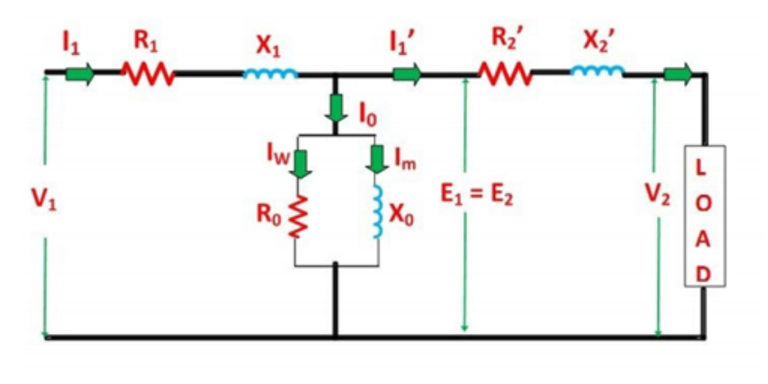
\includegraphics[width=0.5\textwidth]{img6.png}
    \caption{Exact Equivalent Circuit}
\end{figure}\\
For the given transformer, we calculated the absolute parameters as follows:\\
\begin{enumerate}
    \item $R_{0}$=1079.97$\Omega$ \hspace{30mm} 4. $R_{2}$=2.225$\Omega$
    \item $X_{0}$=352.99$\Omega$  \hspace{31.5mm} 5. $X_{1}$=2.681$\Omega$
    \item $R_{1}$=2.225$\Omega$ \hspace{33.5mm} 6. $X_{2}$=2.681$\Omega$
\end{enumerate}
\end{document}
